\section{Motivation}

The previous chapters focused mainly on how an MPC problem is formulated and on which
properties its closed loop may have. We studied nominal MPC, practical extensions, robust
constraint satisfaction, tube MPC, and robustness properties of nominal MPC. In all these cases,
however, one essential issue remains: at every sampling instant the controller must actually
compute a control input.\\
At time \(k\), a general finite-horizon MPC problem has the form
\[
    U_k^\star
    =
    \argmin_{U_k}
    \terminalcost(x_{k+N})
    +
    \sum_{i=0}^{N-1} \stagecost(x_{k+i},u_{k+i})
\]
subject to
\[
    x_k = x(k),
    \qquad
    x_{k+i+1}=g(x_{k+i},u_{k+i}),
\]
and to the constraints
\[
    x_{k+i}\in \cX,\qquad u_{k+i}\in \cU,
    \qquad
    x_{k+N}\in \cX_f .
\]
The optimizer returns an optimal input sequence
\[
    U_k^\star
    =
    \{u_k^\star,u_{k+1}^\star,\ldots,u_{k+N-1}^\star\},
\]
but only the first element \(u_k^\star\) is applied to the plant. At the next sampling instant,
the state is measured again and the optimization problem is solved again.\\
From an implementation point of view, this means that the theoretical MPC law is useful only
if this optimization problem can be solved fast enough and reliably enough for the desired
sampling time. In slow process-control applications, one may have seconds or minutes available.
In fast mechanical or electrical systems, the admissible computation time may be milliseconds,
microseconds, or even less. Thus implementation is not a secondary detail: it is part of the
controller design.\\

There are two main ways to implement the MPC law. The first is to solve the optimization
problem online at every sampling instant using an iterative optimization algorithm. The second
is to solve the parametric optimization problem offline and store the resulting feedback law.
The online computation is then reduced to evaluating a precomputed piecewise affine function.\\

The purpose of this chapter is to explain these two viewpoints. We first discuss explicit MPC,
which exploits the parametric structure of linear MPC problems. Then we discuss iterative
optimization methods, with particular attention to gradient methods, Newton-type methods,
projected-gradient methods, and primal-dual interior-point methods.

\section{Explicit MPC}

\subsection{Parametric viewpoint}

Consider the linear quadratic MPC problem
\[
\begin{aligned}
    U^\star(x(k))
    =
    \argmin_U \quad
    & x_N^\top P x_N
    +
    \sum_{i=0}^{N-1}
    \left(
        x_i^\top Q x_i + u_i^\top R u_i
    \right)
    \\
    \text{subj. to}\quad
    & x_0=x(k),
    \\
    & x_{i+1}=Ax_i+Bu_i,
    \qquad i=0,\ldots,N-1,
    \\
    & x_i\in \cX,\qquad u_i\in \cU,
    \qquad i=0,\ldots,N-1,
    \\
    & x_N\in \cX_f .
\end{aligned}
\]
For a fixed value of \(x(k)\), this is an ordinary quadratic program. However, from the
controller-design viewpoint, \(x(k)\) is not just a number: it is the parameter with respect to
which the controller must be evaluated. The MPC feedback law is therefore the map
\[
    x(k) \mapsto u_0^\star(x(k)).
\]
After eliminating the predicted states, the quadratic-cost CFTOC problem can be written as
\[
    J^\star(x)
    =
    \min_U
    \begin{bmatrix}
        U \\ x
    \end{bmatrix}^{\!\top}
    \begin{bmatrix}
        H & F^\top \\
        F & Y
    \end{bmatrix}
    \begin{bmatrix}
        U \\ x
    \end{bmatrix}
\]
subject to
\[
    GU \leq w + Ex .
\]
This is a multiparametric quadratic program, or mp-QP, where the parameter is the current
state \(x\). The matrices \(H,F,Y,G,w,E\) are fixed offline once the model, horizon, constraints,
and cost weights have been chosen.\\

The central result is that the solution of this parametric problem has a finite polyhedral
structure. The feasible set can be partitioned into polyhedral regions, called critical regions,
and on each region the optimal control law is affine.

\begin{theorembox}[Explicit MPC structure for quadratic-cost linear MPC]
For linear dynamics, polyhedral constraints, and quadratic cost, the MPC problem is an mp-QP.
On the feasible set \(X_N\), the first optimal input has the form
\[
    u_0^\star = \kappa(x),
\]
where
\[
    \kappa(x)=F_jx+g_j
    \qquad \text{if } x\in CR_j,
    \qquad j=1,\ldots,N_r .
\]
The sets
\[
    CR_j=\{x\in\R^n\mid H_jx\leq K_j\}
\]
are polyhedra and form a partition of the feasible set. The value function \(J^\star(x)\) is
convex and piecewise quadratic on the same type of polyhedral partition.
\end{theorembox}

Thus explicit MPC replaces the repeated solution of a QP by the evaluation of a piecewise affine
feedback law. The work is shifted offline: one computes all critical regions and all affine laws in
advance. Online, one only needs to determine which region contains the measured state and then
evaluate the corresponding affine expression.

\subsection{Active sets and critical regions}

The polyhedral regions in explicit MPC are directly related to active sets. To see this, consider
the parametric QP
\[
\begin{aligned}
    \min_U \quad
    & U^\top H U + 2x^\top F U + x^\top Yx
    \\
    \text{subj. to}\quad
    & GU \leq w + Ex.
\end{aligned}
\]
Let
\[
    I:=\{1,\ldots,m_c\}
\]
be the set of indices of all inequality constraints, where \(m_c\) denotes the number of scalar
constraints. For a given parameter \(x\), the active set is the set of constraints that hold with
equality at the optimizer:
\[
    A(x)
    :=
    \{j\in I \mid G_jU^\star(x)-E_jx=w_j\}.
\]
The inactive set is its complement:
\[
    NA(x)
    :=
    \{j\in I \mid G_jU^\star(x)-E_jx<w_j\}.
\]
Here \(G_j\), \(E_j\), and \(w_j\) denote the \(j\)-th row of \(G\), the \(j\)-th row of \(E\), and
the \(j\)-th component of \(w\), respectively.\\

A critical region is the set of parameters for which the optimizer has the same active set.
If \(\bar{x}\) is a feasible parameter and
\[
    A:=A(\bar{x}),
\]
then the corresponding critical region is
\[
    CR_A := \{x\in X_N \mid A(x)=A\}.
\]
Inside such a region, the same constraints are active and inactive. Therefore the KKT system has
the same algebraic structure throughout the whole region. This is the reason why the optimizer
is affine on each critical region.\\

The intuition is the following. If the active constraints are known, then they can be treated
as equalities. Solving the equality-constrained KKT system gives an affine expression in the
parameter \(x\). The region of validity of this expression is then obtained by imposing two
conditions: the inactive constraints must remain inactive, and the Lagrange multipliers of the
active constraints must remain nonnegative. Both conditions are linear inequalities in \(x\),
which explains why the critical regions are polyhedral.

\subsection{A scalar example}

The main idea of parametric programming can already be seen in a one-dimensional example.
Consider
\[
    J^\star(x)
    =
    \min_z
    \left(
        \frac{1}{2}z^2 + 2xz + 2x^2
    \right)
\]
subject to
\[
    z\leq 1+x,
\]
where \(x\in\R\) is a parameter. The goal is to find the optimizer \(z^\star(x)\), the set of
parameters for which the problem has a solution, and the value function \(J^\star(x)\).\\

The Lagrangian is
\[
    L(z,x,\lambda)
    =
    \frac{1}{2}z^2 + 2xz + 2x^2
    +
    \lambda(z-x-1).
\]
The KKT conditions are
\[
    z+2x+\lambda=0,
\]
\[
    z-x-1\leq 0,
\]
\[
    \lambda(z-x-1)=0,
\]
and
\[
    \lambda\geq 0.
\]

There are two possible cases. First, suppose that the constraint is active:
\[
    z-x-1=0.
\]
Then
\[
    z^\star(x)=x+1.
\]
Using stationarity,
\[
    x+1+2x+\lambda=0,
\]
so
\[
    \lambda=-3x-1.
\]
Dual feasibility requires
\[
    -3x-1\geq 0,
\]
and therefore
\[
    x\leq -\frac{1}{3}.
\]
In this region,
\[
    J^\star(x)
    =
    \frac{9}{2}x^2+3x+\frac{1}{2}.
\]
Second, suppose that the constraint is inactive:
\[
    z-x-1<0.
\]
Then \(\lambda=0\), and stationarity gives
\[
    z^\star(x)=-2x.
\]
The inactive constraint condition becomes
\[
    -2x-x-1<0,
\]
or
\[
    x>-\frac{1}{3}.
\]
In this region,
\[
    J^\star(x)=0.
\]
Hence the optimizer is the piecewise affine function
\[
    z^\star(x)
    =
    \begin{cases}
        x+1, & x\leq -\frac{1}{3},\\[2mm]
        -2x, & x\geq -\frac{1}{3},
    \end{cases}
\]
and the value function is
\[
    J^\star(x)
    =
    \begin{cases}
        \dfrac{9}{2}x^2+3x+\dfrac{1}{2},
        & x\leq -\dfrac{1}{3},\\[3mm]
        0,
        & x\geq -\dfrac{1}{3}.
    \end{cases}
\]
This simple example shows the same structure as explicit MPC: different active sets define
different parameter regions, the optimizer is affine on each region, and the value function is
quadratic on each region.

\subsection{Example: double integrator}

A standard example used to visualize explicit MPC is the constrained double integrator
\[
    x(t+1)
    =
    \begin{bmatrix}
        1 & 1\\
        0 & 1
    \end{bmatrix}x(t)
    +
    \begin{bmatrix}
        0\\
        1
    \end{bmatrix}u(t),
\]
with output
\[
    y(t)=
    \begin{bmatrix}
        1 & 0
    \end{bmatrix}x(t).
\]
The system is subject to input constraints
\[
    -1\leq u(k)\leq 1,
    \qquad k=0,\ldots,5,
\]
and state constraints
\[
    \begin{bmatrix}
        -10\\
        -10
    \end{bmatrix}
    \leq
    x(k)
    \leq
    \begin{bmatrix}
        10\\
        10
    \end{bmatrix},
    \qquad k=0,\ldots,5.
\]
One may compute the explicit state-feedback solution for a horizon \(N=6\), weights
\[
    Q=
    \begin{bmatrix}
        1 & 0\\
        0 & 1
    \end{bmatrix},
    \qquad
    R=0.1,
\]
terminal weight \(P\) given by the solution of the algebraic Riccati equation, and terminal set
\[
    \cX_f=\R^2.
\]
The resulting state space is partitioned into finitely many critical regions. In the slide example,
the first optimal input is represented by a piecewise affine surface over the state space. The
important point is not the exact number of regions, but the qualitative structure: the optimal
feedback is not a single linear gain, as in unconstrained LQR. Instead, the constraints divide the
state space into many regions, and the controller has a different affine expression in each of
them.\\

This example also illustrates the main limitation of explicit MPC. Even for a two-dimensional
system and a moderate horizon, the number of regions can already be significant. As the number
of states, inputs, constraints, and horizon length increase, the number of critical regions may
grow very quickly. This growth is one of the main reasons why explicit MPC is mostly limited
to small systems.

\subsection{Norm-based costs}

The same explicit-control idea also applies to MPC problems with \(1\)-norm or \(\infty\)-norm
costs. As discussed in the chapter on constrained finite time optimal control, these problems can
be reformulated as linear programs of the form
\[
    \min_z c^\top z
\]
subject to
\[
    \bar{G}z\leq \bar{w}+\bar{S}x(k).
\]
This is a multiparametric linear program, or mp-LP. Its solution has a structure analogous to
the mp-QP case.

\begin{theorembox}[Explicit MPC structure for norm-based costs]
For linear dynamics, polyhedral constraints, and \(1\)-norm or \(\infty\)-norm costs, the MPC
problem is an mp-LP. A piecewise affine control law exists:
\[
    \kappa(x)=F_jx+g_j
    \qquad \text{if } x\in CR_j.
\]
The feasible set is partitioned into polyhedral critical regions. The value function is convex and
piecewise affine on these regions.
\end{theorembox}

The main difference from the quadratic case is the shape of the value function. With a strictly
convex quadratic cost, the value function is piecewise quadratic and the optimizer is typically
unique. With a linear cost, the value function is piecewise affine and multiple optimizers may
occur. Nevertheless, a piecewise affine feedback law can still be selected.

\section{Online Evaluation of Explicit MPC}

Once an explicit MPC controller has been computed offline, the online task is no longer the
solution of an optimization problem. The controller is already available as a piecewise affine
function of the state. Therefore, at each sampling instant, one only has to evaluate this
piecewise affine map at the current measured state \(x(k)\).\\

More precisely, the explicit control law has the form
\[
    u^\star(x)=F_jx+g_j
    \qquad \text{if } x\in CR_j,
    \qquad j=1,\ldots,N_r,
\]
where the critical regions
\[
    CR_j=\{x\in\R^n\mid H_jx\leq K_j\}
\]
form a polyhedral partition of the feasible set. Hence the online evaluation naturally separates
into two steps. First, one has to determine which critical region contains the current state.
Second, once the correct region has been found, one evaluates the corresponding affine control
law.\\
The important observation is that the affine evaluation itself is very cheap: it only requires a
matrix-vector multiplication and an addition. Thus the computational bottleneck is usually not
the formula
\[
    u(k)=F_jx(k)+g_j,
\]
but rather the point-location problem:
\[
    \text{find } j \text{ such that } x(k)\in CR_j.
\]
On a boundary between two critical regions, more than one region may contain the same state.
For quadratic-cost explicit MPC, the control law is continuous, so this ambiguity does not
change the applied input.

\subsection{Sequential search}

The most direct way to solve the point-location problem is sequential search. Each critical
region is tested one after the other until the region containing the current state is found. If the
regions are stored as
\[
    CR_j=\{x\in\R^n\mid A_jx+b_j\leq 0\},
\]
then the algorithm is simply
\[
\begin{array}{ll}
    \text{for each } j: & \\
    & \text{if } A_jx+b_j\leq 0, \text{ then } x \text{ is in region } j .
\end{array}
\]
Once the correct region has been found, the corresponding affine law is evaluated.

\begin{figure}[!h]
    \centering
    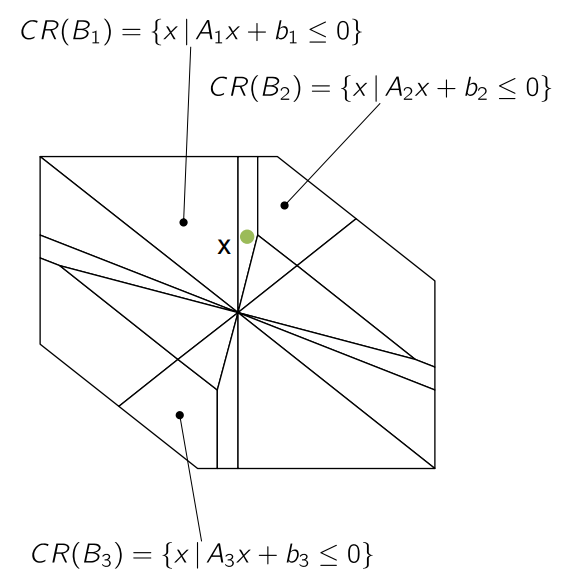
\includegraphics[width=0.5\textwidth]{images/sequential_search.png}
    \caption{Sequential search for point location. The regions are checked one by one by
    testing their defining inequalities. The method is very simple and works for arbitrary
    explicit MPC partitions, but its online cost grows linearly with the number of regions.}
    \label{fig:explicit_mpc_sequential_search}
\end{figure}

The advantage of sequential search is its simplicity. It requires almost no additional offline
processing beyond storing the polyhedral regions themselves, and it works for all explicit MPC
problems. The disadvantage is that, in the worst case, all regions may have to be tested before
the correct one is found. Therefore, if the explicit solution contains \(N_r\) regions, the online
complexity is proportional to
\[
    N_r .
\]
This is acceptable for small explicit controllers, but it becomes inefficient when the number of
critical regions is large.

\subsection{Logarithmic search}

A faster method can be obtained by constructing a search tree offline. The idea is to avoid
testing the regions one by one. Instead, one chooses a hyperplane that separates the set of
regions into two groups of roughly equal size. Then the same procedure is repeated recursively
on the two subsets. In this way, the offline phase builds a binary decision tree.\\
At each node of the tree, the online controller only has to test on which side of a separating
hyperplane the current state lies. For example, if the separating hyperplane is described by
\[
    h^\top x+c=0,
\]
then the test is
\[
    h^\top x+c\leq 0
    \qquad \text{or} \qquad
    h^\top x+c>0.
\]
The result determines whether the search continues in the left or in the right branch of the
tree.

\begin{figure}[!h]
    \centering
    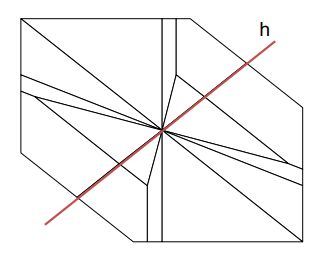
\includegraphics[width=0.4\textwidth]{images/log_search_1.png}
    \caption{Offline construction of a search tree. A separating hyperplane is chosen so as to
    split the set of critical regions into two subsets of comparable size. The same construction
    is then repeated recursively on the two subsets.}
    \label{fig:explicit_mpc_log_search_1}
\end{figure}

The online procedure is then very similar to a binary search. Starting from the root node, the
current state is tested against the first separating hyperplane. This discards approximately half
of the candidate regions. A second hyperplane is then tested in the remaining subset, discarding
again a large portion of the remaining candidates. Repeating this process leads to a leaf of the
tree, which identifies the critical region containing the state.

\begin{figure}[!h]
    \centering
    \begin{subfigure}{0.48\textwidth}
        \centering
        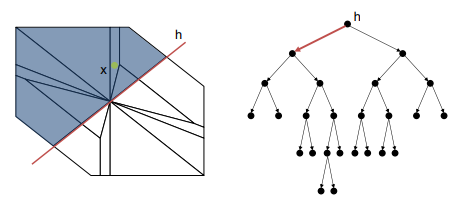
\includegraphics[width=\textwidth]{images/log_search_2.png}
        \caption{First test at the root node.}
        \label{fig:explicit_mpc_log_search_2}
    \end{subfigure}
    \hfill
    \begin{subfigure}{0.48\textwidth}
        \centering
        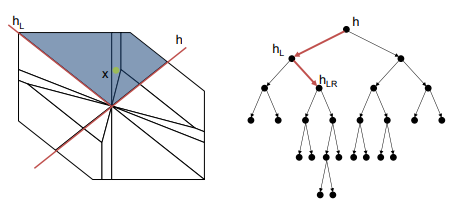
\includegraphics[width=\textwidth]{images/log_search_3.png}
        \caption{Second test in the selected branch.}
        \label{fig:explicit_mpc_log_search_3}
    \end{subfigure}

    \vspace{0.4cm}

    \begin{subfigure}{0.48\textwidth}
        \centering
        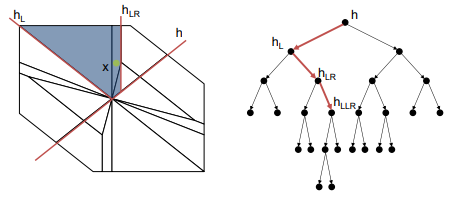
\includegraphics[width=\textwidth]{images/log_search_4.png}
        \caption{Further refinement of the candidate set.}
        \label{fig:explicit_mpc_log_search_4}
    \end{subfigure}
    \hfill
    \begin{subfigure}{0.48\textwidth}
        \centering
        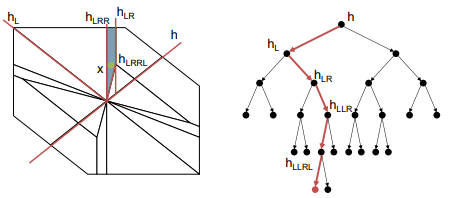
\includegraphics[width=\textwidth]{images/log_search_6.png}
        \caption{The leaf node identifies the final region.}
        \label{fig:explicit_mpc_log_search_6}
    \end{subfigure}

    \caption{Logarithmic search for explicit MPC. The left part of each slide shows the
    progressive localization of the state in the polyhedral partition. The right part shows the
    corresponding path in the binary search tree. Each hyperplane test eliminates a large subset
    of candidate regions.}
    \label{fig:explicit_mpc_logarithmic_search}
\end{figure}

If the tree is well balanced, the number of online tests grows approximately as
\[
    \log_2(N_r),
\]
rather than as \(N_r\). This is the reason for the name logarithmic search. The improvement can
be substantial when the explicit controller contains many regions.\\
The price to pay is offline complexity. The search tree must be built before the controller is
implemented. This requires selecting separating hyperplanes, organizing the regions into a tree,
and storing the resulting data structure. Therefore logarithmic search is most useful when the
explicit controller is not too large to preprocess, but large enough that sequential search would
be inefficient. In practice, this is reasonable for explicit controllers with up to roughly a few
hundred or a few thousand regions, depending on the implementation platform and memory
constraints.

\subsection{Summary of explicit MPC implementation}

The main advantage of explicit MPC is that the optimization problem is solved before runtime.
For linear MPC with polyhedral constraints and quadratic or linear-norm costs, the controller is
piecewise affine. Therefore, after offline computation, the online controller only evaluates a
piecewise affine function.\\
The online evaluation is extremely fast. Once the correct critical region is known, the input is
computed as
\[
    u(k)=F_jx(k)+g_j.
\]
This can often be done in nanoseconds or microseconds on suitable hardware. This makes
explicit MPC attractive for applications with very small sampling times.\\
However, explicit MPC is limited by the size of the polyhedral partition. As the state dimension,
input dimension, horizon length, and number of constraints increase, the number of regions may
grow very quickly. The controller may then become too expensive to compute offline, too large
to store, or too slow to evaluate by point location. For this reason, explicit MPC is mainly used
for small systems, typically with a few states.\\

In summary, explicit MPC replaces online optimization by offline parametric optimization and
online point location. This is extremely effective for small problems, but online optimization
methods are usually preferable for medium- and large-scale MPC problems.

\section{Iterative Numerical Optimization}

\subsection{Why numerical methods are needed}

Explicit MPC shifts the computational burden offline, but this is not always possible. In most
practical MPC applications, the optimization problem is solved online at every sampling instant.
This requires efficient numerical optimization algorithms.\\

Recall the general convex optimization problem
\[
\begin{aligned}
    \min_x \quad & f(x)\\
    \text{subj. to}\quad & x\in Q.
\end{aligned}
\]
The problem is convex if \(f\) and \(Q\) are convex. The most important special cases for MPC
are linear programs,
\[
\begin{aligned}
    \min_x \quad & c^\top x\\
    \text{subj. to}\quad & Ax=b,\\
    & Gx\leq h,
\end{aligned}
\]
and quadratic programs,
\[
\begin{aligned}
    \min_x \quad & \frac{1}{2}x^\top Hx+c^\top x\\
    \text{subj. to}\quad & Ax=b,\\
    & Gx\leq h,
\end{aligned}
\]
where the QP is convex if
\[
    H\succeq 0.
\]
In all but the simplest cases, an analytical optimizer cannot be written down explicitly. A
numerical method therefore starts from an initial guess \(x^{(0)}\) and produces a sequence of
iterates
\[
    x^{(i+1)}
    =
    \Psi(x^{(i)},f,Q),
    \qquad i=0,1,\ldots,m-1.
\]
The goal is to obtain an approximate solution \(x^{(m)}\) satisfying
\[
    |f(x^{(m)})-f(x^\star)|\leq \varepsilon
\]
and
\[
    \operatorname{dist}(x^{(m)},Q)\leq \delta,
\]
where \(\varepsilon\) and \(\delta\) are tolerances chosen by the user.\\
In MPC, these tolerances have a control interpretation. Solving the optimization problem only
approximately means that the applied input may not be exactly optimal, and may even be slightly
infeasible if constraint tolerances are not handled carefully. Therefore solver accuracy,
computation time, and closed-loop performance are directly linked.

\section{Unconstrained Minimization}

We now turn to the first family of iterative optimization methods. Before considering constrained
problems, it is useful to understand the simpler unconstrained case
\[
    \min_x f(x),
    \qquad
    f:\R^n\to\R.
\]
Throughout this section we assume that \(f\) is convex and twice continuously differentiable,
and that the optimal value
\[
    p^\star=\min_x f(x)
\]
is finite. These assumptions are stronger than what is needed for all algorithms, but they allow
us to present the main ideas cleanly.\\
For unconstrained convex minimization, optimality is characterized by a very simple condition.
If \(f\) is differentiable, then a point \(x^\star\) is a global minimizer if and only if
\[
    \nabla f(x^\star)=0.
\]
Thus the problem of minimizing \(f\) can be interpreted as the problem of solving the nonlinear
system of equations
\[
    \nabla f(x)=0.
\]
In general, this system has no closed-form analytical solution. Numerical methods therefore
construct a sequence of iterates that hopefully converges to a point satisfying this optimality
condition.

\begin{theorembox}[Necessary and sufficient optimality condition]
Assume that \(f\) is convex and differentiable. Then
\[
    x^\star\in\argmin_x f(x)
    \qquad \Longleftrightarrow \qquad
    \nabla f(x^\star)=0.
\]
Unconstrained minimization methods can therefore be interpreted as iterative methods for
solving the optimality condition \(\nabla f(x^\star)=0\).
\end{theorembox}

\subsection{Descent methods}

The basic idea behind descent methods is to move from the current iterate to a new point with
a smaller objective value. Starting from \(x^{(i)}\), one chooses a step, or search direction,
\(\Delta x^{(i)}\), and a step size, or step length, \(h^{(i)}>0\). The next iterate is then
defined by
\[
    x^{(i+1)}
    =
    x^{(i)}+h^{(i)}\Delta x^{(i)}.
\]
The direction \(\Delta x^{(i)}\) is called a descent direction if the step can be chosen so that
\[
    f(x^{(i+1)})<f(x^{(i)}).
\]
A useful sufficient condition is
\[
    \nabla f(x^{(i)})^\top \Delta x^{(i)}<0.
\]
Indeed, the quantity \(\nabla f(x^{(i)})^\top \Delta x^{(i)}\) is the directional derivative of
\(f\) at \(x^{(i)}\) in the direction \(\Delta x^{(i)}\). If this number is negative, then moving a
small enough positive distance in that direction decreases the objective.

A general descent method has the following structure:
\[
\begin{array}{ll}
\textbf{Input:} & \text{starting point } x^{(0)}\in\operatorname{dom} f,\\[1mm]
\textbf{repeat} & \\
& 1.\ \text{Compute a descent direction } \Delta x^{(i)},\\
& 2.\ \text{Choose a step size } h^{(i)}>0 \text{ such that}\\
& \qquad f(x^{(i)}+h^{(i)}\Delta x^{(i)})<f(x^{(i)}),\\
& 3.\ \text{Update } x^{(i+1)}:=x^{(i)}+h^{(i)}\Delta x^{(i)},\\[1mm]
\textbf{until} & \text{a termination condition is satisfied.}
\end{array}
\]
Typical stopping criteria are based on the objective decrease or on the change between
successive iterates, for instance
\[
    f(x^{(m)})-f(x^\star)\leq \varepsilon_1
    \qquad \text{or} \qquad
    \norm{x^{(m)}-x^{(m-1)}}\leq \varepsilon_2.
\]
In practice, \(f(x^\star)\) is usually not known, so stopping conditions are often expressed in
terms of computable quantities such as gradient norms, primal and dual residuals, or relative
changes in the objective.

\subsection{Gradient method}

The simplest way to choose a descent direction is to use the gradient. Since \(\nabla f(x)\)
points in the direction of steepest local ascent, the negative gradient points in the direction of
steepest local descent. The gradient descent update is therefore
\[
    x^{(i+1)}
    =
    x^{(i)}-h^{(i)}\nabla f(x^{(i)}).
\]
This formula has an immediate interpretation: at each iteration, one moves against the local
slope of the objective. The remaining question is how to choose the step size \(h^{(i)}\). If the
step is too small, convergence is slow. If the step is too large, the method may overshoot and
increase the objective.

A standard way to obtain a safe constant step size is to assume that \(f\) is \(L\)-smooth. This
means that the gradient is Lipschitz continuous with constant \(L\):
\[
    \norm{\nabla f(x)-\nabla f(y)}
    \leq
    L\norm{x-y},
    \qquad
    \forall x,y\in\R^n.
\]
Equivalently, \(f\) can be upper bounded by a quadratic approximation:
\[
    f(x)
    \leq
    f(y)+\nabla f(y)^\top(x-y)
    +
    \frac{L}{2}\norm{x-y}^2,
    \qquad
    \forall x,y\in\R^n.
\]
This inequality says that, around every point \(y\), the function lies below a quadratic model
with curvature \(L\). The larger \(L\) is, the more conservative the step size must be.

\begin{figure}[!h]
    \centering
    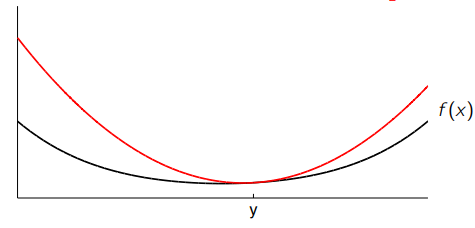
\includegraphics[width=0.5\textwidth]{images/l_smoothness_constant_step.png}
    \caption{\(L\)-smoothness and constant step size. If the gradient is Lipschitz continuous
    with constant \(L\), the function can be upper bounded by a quadratic model. This motivates
    the constant step size \(h^{(i)}=1/L\).}
    \label{fig:l_smoothness_constant_step}
\end{figure}

Under this smoothness assumption, a natural constant choice is
\[
    h^{(i)}=\frac{1}{L}.
\]
The main advantage of gradient descent is that each iteration is cheap: only the gradient has to
be evaluated. The main disadvantage is that many iterations may be needed, especially for
ill-conditioned problems. This is important in MPC, where one must often trade cheap iterations
against the strict real-time requirement imposed by the sampling period.

\subsection{Newton's method}

Newton's method chooses the search direction in a more sophisticated way. Instead of using only
the first-order information contained in the gradient, it builds a second-order approximation of
the objective around the current iterate \(x^{(i)}\). The local quadratic model is
\[
\begin{aligned}
    \tilde f(x,x^{(i)})
    =
    f(x^{(i)})
    &+
    \nabla f(x^{(i)})^\top (x-x^{(i)})
    \\
    &+
    \frac{1}{2}
    (x-x^{(i)})^\top
    \nabla^2 f(x^{(i)})
    (x-x^{(i)}).
\end{aligned}
\]
Newton's idea is to minimize this second-order approximation:
\[
    x^{(i+1)}
    =
    \argmin_x \tilde f(x,x^{(i)}).
\]

\begin{figure}[!h]
    \centering
    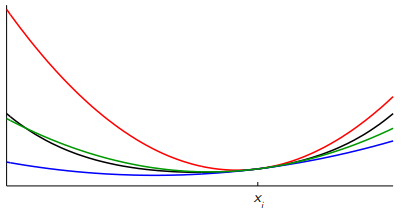
\includegraphics[width=0.5\textwidth]{images/newton_quadratic_approximation.png}
    \caption{Newton's method. At the current iterate \(x^{(i)}\), the function is approximated
    by a second-order Taylor model. The Newton step minimizes this local quadratic model.
    Unlike the \(L\)-smoothness upper bound, this quadratic approximation is not necessarily a
    global upper bound on \(f\).}
    \label{fig:newton_quadratic_approximation}
\end{figure}

The first-order condition for the minimizer of the quadratic model is
\[
    \nabla_x \tilde f(x,x^{(i)})\big|_{x=x^{(i+1)}}=0.
\]
Computing the derivative gives
\[
    \nabla f(x^{(i)})
    +
    \nabla^2 f(x^{(i)})(x^{(i+1)}-x^{(i)})
    =
    0.
\]
Therefore,
\[
    x^{(i+1)}
    =
    x^{(i)}
    -
    \left(\nabla^2 f(x^{(i)})\right)^{-1}
    \nabla f(x^{(i)}).
\]
The corresponding Newton direction is
\[
    \Delta x_{\mathrm{nt}}^{(i)}
    =
    -
    \left(\nabla^2 f(x^{(i)})\right)^{-1}
    \nabla f(x^{(i)}).
\]
Hence the full Newton update can be written as
\[
    x^{(i+1)}=x^{(i)}+\Delta x_{\mathrm{nt}}^{(i)}.
\]
However, the quadratic model \(\tilde f\) is not necessarily an upper bound on \(f\). Therefore,
a full Newton step does not always decrease the original objective. It may happen that
\[
    f(x^{(i+1)})>f(x^{(i)}),
\]
especially when the current iterate is far from the minimizer. For this reason, one often uses a
damped Newton step:
\[
    x^{(i+1)}
    =
    x^{(i)}
    +
    h^{(i)}\Delta x_{\mathrm{nt}}^{(i)}
    =
    x^{(i)}
    -
    h^{(i)}
    \left(\nabla^2 f(x^{(i)})\right)^{-1}
    \nabla f(x^{(i)}),
\]
where \(h^{(i)}>0\) is chosen so that the step yields descent.\\
Newton's method is more expensive per iteration than gradient descent because it requires the
Hessian and the solution of a linear system. On the other hand, when the iterate is sufficiently
close to the optimum, Newton's method can converge much faster. This is one of the reasons why
Newton-type ideas appear inside many high-performance optimization algorithms for MPC.

\subsection{Line search}

The step size in a descent method is often computed by line search. Given a direction
\(\Delta x\), for instance the Newton direction \(\Delta x_{\mathrm{nt}}\), one wants to find
\[
    h^{(i)}>0
\]
such that
\[
    f(x^{(i)}+h^{(i)}\Delta x_{\mathrm{nt}})
    <
    f(x^{(i)}).
\]
The most direct possibility is exact line search, where one solves the one-dimensional
optimization problem
\[
    h^{(i)\star}
    =
    \argmin_{h>0}
    f(x^{(i)}+h\Delta x_{\mathrm{nt}}).
\]
This gives the best step size along the chosen direction. However, it can be time consuming
because it may require many evaluations of \(f\). For this reason, exact line search is often not
the preferred choice in real-time MPC algorithms.\\

A cheaper alternative is inexact line search. The goal is not to find the best step size, but only
to find a step size that decreases the objective by a sufficient amount. A standard example is
backtracking line search. Choose parameters
\[
    \alpha\in(0,0.5),
    \qquad
    \beta\in(0,1).
\]
Initialize
\[
    h^{(i)}=1.
\]
Then repeat the update
\[
    h^{(i)}\leftarrow \beta h^{(i)}
\]
as long as
\[
    f(x^{(i)}+h^{(i)}\Delta x_{\mathrm{nt}})
    >
    f(x^{(i)})
    +
    \alpha h^{(i)}
    \nabla f(x^{(i)})^\top \Delta x_{\mathrm{nt}}.
\]
Once this inequality is no longer true, the step size is accepted. This condition is known as a
sufficient-decrease condition. It guarantees that the step is not merely decreasing the objective,
but decreasing it by an amount compatible with the local slope in the chosen direction.

\subsection{Equality constraints in Newton's method}

Newton's method can also be adapted to equality-constrained problems. Consider
\[
\begin{aligned}
    \min_x \quad & f(x)\\
    \text{subj. to}\quad & Ax=b,
\end{aligned}
\]
where \(A\in\R^{m\times n}\). At the current iterate \(x^{(i)}\), the Newton direction is obtained
by minimizing the quadratic model of \(f\) subject to the equality constraint on the next
iterate. Written in terms of the step \(\Delta x\), this gives
\[
\begin{aligned}
    \Delta x_{\mathrm{nt}}(x^{(i)})
    \in
    \argmin_{\Delta x}\quad
    &
    \frac{1}{2}
    \Delta x^\top
    \nabla^2 f(x^{(i)})
    \Delta x
    +
    \nabla f(x^{(i)})^\top \Delta x
    \\
    \text{subj. to}\quad
    &
    A\Delta x=-Ax^{(i)}+b.
\end{aligned}
\]
If the current iterate is feasible, namely
\[
    Ax^{(i)}=b,
\]
then the constraint on the Newton direction becomes
\[
    A\Delta x=0.
\]
Thus the Newton direction lies in the null space of \(A\). Consequently, for any step size
\(h^{(i)}\),
\[
\begin{aligned}
    Ax^{(i+1)}
    &=
    A\left(x^{(i)}+h^{(i)}\Delta x_{\mathrm{nt}}\right)\\
    &=
    Ax^{(i)}+h^{(i)}A\Delta x_{\mathrm{nt}}\\
    &=
    b.
\end{aligned}
\]
Therefore, if the initial iterate is feasible, all subsequent iterates remain feasible.\\
The computation of the equality-constrained Newton direction amounts to solving a linear
system of equations. The optimality conditions of the quadratic subproblem, with multiplier
\(\nu\in\R^m\), are
\[
    \nabla^2 f(x^{(i)})\Delta x
    +
    \nabla f(x^{(i)})
    +
    A^\top \nu
    =
    0,
\]
\[
    A\Delta x=0.
\]
Equivalently,
\[
    \begin{bmatrix}
        \nabla^2 f(x^{(i)}) & A^\top\\
        A & 0
    \end{bmatrix}
    \begin{bmatrix}
        \Delta x\\
        \nu
    \end{bmatrix}
    =
    \begin{bmatrix}
        -\nabla f(x^{(i)})\\
        0
    \end{bmatrix}.
\]
This saddle-point system is an important building block for constrained optimization. In
particular, closely related KKT systems appear in interior-point methods and active-set methods
for the quadratic programs that arise in MPC.

\section{Constrained Minimization}

We now move from unconstrained minimization to constrained optimization. This is the setting
that is most relevant for MPC, since the finite-horizon problem contains input constraints, state
constraints, and often terminal constraints. In the convex case, the most common numerical
methods can be grouped into three broad families.\\

Gradient-descent methods are based on the same idea as in the unconstrained case: the gradient
gives the direction of steepest local ascent, so one tries to move in the anti-gradient direction.
The main difference is that the constraints must now be respected. This can be done, for
example, by projecting the tentative gradient step back onto the feasible set.

Interior-point methods take a different viewpoint. Instead of explicitly guessing which
constraints will be active at the solution, they solve a sequence of relaxed KKT systems. These
systems are usually solved using Newton's method. As the relaxation is reduced, the iterates
approach the true constrained optimum.

Active-set methods are based on the idea that the main difficulty is to identify which inequality
constraints are active at the optimum. If the active set were known, the problem would locally
reduce to an equality-constrained optimization problem. Active-set methods therefore try to
identify this set iteratively. This is especially useful for MPC QPs, because consecutive problems
are often similar and the active set from the previous sampling instant can be used as a warm
start.

\subsection{Projected gradient method}

Consider the constrained convex optimization problem
\[
\begin{aligned}
    \min_x \quad & f(x)\\
    \text{subj. to}\quad & x\in Q,
\end{aligned}
\tag{P}
\]
where \(Q\) is a convex set and \(f\) is convex and \(L\)-smooth. In unconstrained gradient
descent, one would take the step
\[
    x^{(i)}-\frac{1}{L}\nabla f(x^{(i)}).
\]
With constraints, this tentative point may lie outside the feasible set. The projected-gradient
method therefore incorporates the constraints by projecting the tentative step back onto \(Q\):
\[
    x^{(i+1)}
    =
    \pi_Q
    \left(
        x^{(i)}-h^{(i)}\nabla f(x^{(i)})
    \right).
\]
Here \(\pi_Q\) denotes the Euclidean projection onto \(Q\), defined as
\[
    \pi_Q(y)
    :=
    \argmin_x
    \frac{1}{2}\norm{x-y}_2^2
    \qquad
    \text{subj. to } x\in Q.
\]
Thus the method has a very intuitive interpretation. First, one moves in the anti-gradient
direction, exactly as in the unconstrained case. Then, if the tentative point is infeasible, one
replaces it by the closest feasible point.

\begin{figure}[!h]
    \centering
    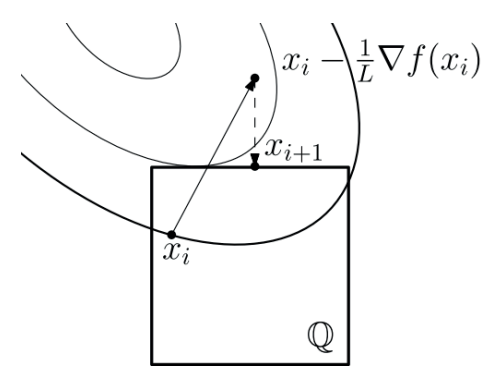
\includegraphics[width=0.4\textwidth]{images/projected_gradient_method.png}
    \caption{Projected-gradient method for constrained minimization. The method first takes an
    unconstrained gradient step and then projects the result back onto the feasible set \(Q\).
    The projection \(\pi_Q(y)\) is the closest feasible point to the tentative point \(y\).}
    \label{fig:projected_gradient_method}
\end{figure}

If \(f\) is \(L\)-smooth, one can choose the same constant step size as in the unconstrained
case,
\[
    h^{(i)}=\frac{1}{L}.
\]
The convergence rates are then analogous to those of the unconstrained gradient method, at
least when the projection can be computed efficiently.\\
The practical usefulness of projected gradient depends almost entirely on the projection. If
\(Q\) is simple, such as a box, a ball, or another set with a closed-form projection, then the
method is very attractive. If \(Q\) is a complicated polyhedron or an intersection of many coupled
constraints, then computing \(\pi_Q\) may itself require solving a nontrivial optimization problem.
In that case, the simplicity of the method can be lost.

\subsection{Implications for MPC}

The projected-gradient idea has a direct interpretation in MPC. Consider first a condensed MPC
formulation in which the predicted states have been eliminated and the only decision variable is
the stacked input vector \(u\). If the only constraints are simple input constraints, then the
problem may have the form
\[
\begin{aligned}
    \min_u \quad
    &
    \frac{1}{2}u^\top H u + x_0^\top F u
    \\
    \text{subj. to}\quad
    &
    u\in \cU.
\end{aligned}
\]
If \(\cU\) is a simple set, for example a box constraint on the inputs, then projection onto
\(\cU\) is cheap. Projected-gradient methods are then natural: one takes a gradient step in the
input sequence and projects the result back onto the admissible input set.\\

The situation becomes more subtle when state constraints are present. In a sparse formulation,
one keeps both states and inputs as decision variables and writes
\[
    z:=(x,u).
\]
The simple constraints can be collected into the product set
\[
    K:=\cX\times\cU.
\]
Projection onto \(K\) may be easy if \(\cX\) and \(\cU\) are simple sets. However, the dynamics
also impose equality constraints of the form
\[
    Az=b,
\]
where this compact equation represents the stacked system dynamics and the initial condition.
The true feasible set is therefore
\[
    K\cap \{z\mid Az=b\}.
\]
Even if projection onto \(K\) is easy and projection onto the affine set \(\{z\mid Az=b\}\) is
manageable, projection onto their intersection is generally not easy.

\begin{figure}[!h]
    \centering
    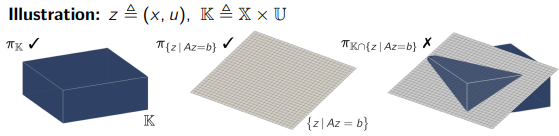
\includegraphics[width=0.88\textwidth]{images/projected_gradient_mpc_implications.png}
    \caption{Implications of projected-gradient methods for MPC. With simple input constraints
    in a condensed formulation, projections may be cheap. With state constraints and dynamics,
    the feasible set becomes an intersection between simple constraint sets and the affine
    dynamics constraint, and projection onto the intersection is no longer straightforward.}
    \label{fig:projected_gradient_mpc_implications}
\end{figure}

This explains why the formulation of the MPC problem matters so much. A condensed formulation
may lead to a smaller problem, but it can destroy sparsity. A sparse formulation preserves the
dynamical structure, but it introduces equality constraints and coupled feasibility conditions.
Depending on the problem, one may prefer primal methods, dual methods, projected-gradient
methods, interior-point methods, or active-set methods.\\
In the presence of state constraints, one common strategy is to dualize some constraints or the
dynamics. The resulting algorithms do not require projection onto the full intersection directly;
instead, they alternate between simpler primal operations and dual updates. The key message is
that first-order methods are attractive for MPC only when the constraint handling can be made
cheap.

\section{Interior-Point Methods}

\subsection{Constrained problem and KKT conditions}

We now consider interior-point methods. The starting point is a constrained convex optimization
problem with inequality and equality constraints:
\[
\begin{aligned}
    \min_x \quad & f(x)\\
    \text{subj. to}\quad
    & g_i(x)\leq 0,
    \qquad i=1,\ldots,m,
    \\
    & Cx=d.
\end{aligned}
\]
We assume that \(f\) and the functions \(g_i\) are convex and twice continuously differentiable.
We also assume that the optimal value \(f(x^\star)\) is finite and attained, that the feasible set
is closed and compact, and that strict feasibility holds. Strict feasibility means that there
exists a point \(\tilde{x}\) such that
\[
    \tilde{x}\in\operatorname{dom} f,
    \qquad
    g_i(\tilde{x})<0,
    \qquad i=1,\ldots,m,
\]
and
\[
    C\tilde{x}=d.
\]
Under these assumptions, the KKT conditions can be used to characterize optimality.

To prepare the problem for a primal-dual interior-point method, we introduce slack variables
\[
    s\in\R^m,
    \qquad
    s_i\geq 0.
\]
The inequalities are rewritten as equalities:
\[
    g_i(x)+s_i=0,
    \qquad i=1,\ldots,m.
\]
The standard KKT conditions then consist of stationarity,
\[
    \nabla f(x^\star)
    +
    \sum_{i=1}^m
    \lambda_i^\star \nabla g_i(x^\star)
    +
    C^\top \nu^\star
    =
    0,
\]
primal feasibility,
\[
    Cx^\star=d,
    \qquad
    g_i(x^\star)+s_i^\star=0,
    \qquad i=1,\ldots,m,
\]
dual feasibility,
\[
    \lambda_i^\star\geq 0,
    \qquad
    s_i^\star\geq 0,
\]
and complementarity,
\[
    \lambda_i^\star s_i^\star=0,
    \qquad i=1,\ldots,m.
\]
Complementarity is the difficult part. At the optimum, for each inequality constraint, either
the slack is positive and the multiplier is zero, or the slack is zero and the multiplier may be
positive. Thus complementarity encodes the active-set structure of the solution.

\subsection{Primal-dual interior-point idea}

Interior-point methods avoid deciding explicitly which constraints are active. Instead, they
replace the exact complementarity condition
\[
    \lambda_i s_i=0
\]
by a relaxed condition
\[
    \lambda_i s_i=\kappa,
    \qquad \kappa>0.
\]
Equivalently, in the notation of the slides, the relaxed system is written as
\[
\begin{aligned}
    \nabla f(x^\star)
    +
    \sum_{i=1}^{m}\lambda_i^\star\nabla g_i(x^\star)
    +
    C^\top \nu^\star
    &=0,\\
    Cx^\star&=d,\\
    g_i(x^\star)+s_i^\star&=0,
    \qquad i=1,\ldots,m,\\
    \lambda_i^\star g_i(x^\star)&=-\kappa,
    \qquad i=1,\ldots,m,\\
    \lambda_i^\star,\ s_i^\star&\geq 0,
    \qquad i=1,\ldots,m.
\end{aligned}
\tag{**}
\]
The form \(\lambda_i^\star g_i(x^\star)=-\kappa\) is equivalent to
\(\lambda_i^\star s_i^\star=\kappa\), since \(g_i(x^\star)+s_i^\star=0\).

For a fixed positive value of \(\kappa\), the solution of the relaxed equations lies strictly in
the interior with respect to the nonnegativity constraints:
\[
    \lambda_i>0,
    \qquad
    s_i>0.
\]
As \(\kappa\) is reduced toward zero, the relaxed solution approaches the true KKT point. The
set of relaxed solutions obtained for different positive values of \(\kappa\) is called the
primal-dual central path:
\[
    \mathcal{C}
    :=
    \{(x,\nu,\lambda,s)\mid (**) \text{ holds for some } \kappa>0\}.
\]
A primal-dual interior-point method follows this central path toward the optimum while
gradually reducing \(\kappa\).

The word primal-dual emphasizes that the method solves for the primal variables \(x\), the
equality multipliers \(\nu\), the inequality multipliers \(\lambda\), and the slack variables \(s\)
simultaneously. The relaxed KKT system is solved by Newton's method, together with additional
safeguards and line search to preserve positivity and to ensure progress.

\begin{theorembox}[Interior-point principle]
Primal-dual interior-point methods solve the primal and dual problems simultaneously by
following the relaxed KKT equations. The complementarity condition is relaxed from
\(\lambda_i s_i=0\) to \(\lambda_i s_i=\kappa\), and \(\kappa\) is reduced to zero as the method
approaches the optimum.
\end{theorembox}

\subsection{Primal-dual search direction}

At each iteration, the relaxed KKT system is linearized and a Newton direction is computed.
Define
\[
    S:=\operatorname{diag}(s_1,\ldots,s_m),
    \qquad
    \Lambda:=\operatorname{diag}(\lambda_1,\ldots,\lambda_m),
\]
and
\[
    G(x)^\top
    :=
    \begin{bmatrix}
        \nabla g_1(x) & \cdots & \nabla g_m(x)
    \end{bmatrix}.
\]
The Hessian of the Lagrangian with respect to \(x\) is
\[
    H(x,\lambda)
    :=
    \nabla^2 f(x)
    +
    \sum_{i=1}^{m}
    \lambda_i\nabla^2 g_i(x).
\]
Linearizing the relaxed KKT equations gives the Newton system
\[
\begin{bmatrix}
    H(x,\lambda) & C^\top & G(x)^\top & 0\\
    C            & 0      & 0        & 0\\
    G(x)         & 0      & 0        & I\\
    0            & 0      & S        & \Lambda
\end{bmatrix}
\begin{bmatrix}
    \Delta x\\
    \Delta \nu\\
    \Delta \lambda\\
    \Delta s
\end{bmatrix}
=
-
\begin{bmatrix}
    \nabla f(x)+C^\top\nu+G(x)^\top\lambda\\
    Cx-d\\
    g(x)+s\\
    S\lambda-v
\end{bmatrix}.
\]
The vector \(v\in\R^m\) modifies the right-hand side of the complementarity equation. We denote
the resulting direction by
\[
    \Delta [x,\nu,\lambda,s](v).
\]
Different choices of \(v\) give different search directions.

If
\[
    v=0,
\]
one obtains the pure Newton direction for the uncentered complementarity equations. This is
often called the predictor direction or affine-scaling direction. It points aggressively toward
the boundary and predicts how the method would move if it tried to reduce complementarity
rapidly.

If
\[
    v=\kappa \mathbf{1},
\]
one obtains a centering direction. This direction pulls the iterate toward the central path,
preventing it from approaching the boundary too aggressively.

In practice, primal-dual methods combine these ideas. One chooses
\[
    v=\sigma\kappa\mathbf{1},
    \qquad
    \sigma\in(0,1),
\]
where \(\sigma\) is a centering parameter. This gives a search direction that both reduces
complementarity and keeps the iterates sufficiently close to the central path.

\begin{figure}[!h]
    \centering
    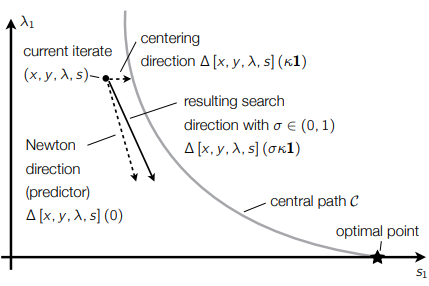
\includegraphics[width=0.6\textwidth]{images/primal_dual_search_directions.png}
    \caption{Search directions in primal-dual interior-point methods. The predictor direction
    aims toward the optimum by reducing complementarity aggressively. The centering direction
    pulls the iterate back toward the central path. Practical methods combine the two effects
    using a centering parameter \(\sigma\in(0,1)\).}
    \label{fig:primal_dual_search_directions}
\end{figure}

After computing the direction, a step size must be chosen. The step cannot be arbitrary, because
the method must preserve
\[
    s+\alpha\Delta s>0,
    \qquad
    \lambda+\alpha\Delta\lambda>0.
\]
Therefore the Newton direction is combined with a line search and additional safeguards. The
goal is to decrease residuals and complementarity while remaining in the interior of the
nonnegative orthant.

\subsection{Interior-point methods in MPC}

Interior-point methods are widely used in MPC because the optimization problems arising from
linear MPC are typically LPs or QPs with a highly structured KKT system. In a sparse MPC
formulation, the equality constraints come from the dynamics over the prediction horizon.
Consequently, the Newton systems have a block structure that can be exploited computationally.\\

The main strength of interior-point methods is that they handle many inequality constraints
without explicitly identifying the active set. This makes them robust and reliable for large
convex optimization problems. The main computational cost is the solution of a linear system at
each Newton step. Therefore, efficient MPC implementations exploit sparsity, block structure,
fixed horizon dimensions, and warm starts whenever possible.\\
From the MPC viewpoint, interior-point methods are attractive when the problem is too large for
explicit MPC and when one wants a reliable online solver. They are especially effective when the
solver is tailored to the optimal-control structure rather than treating the MPC problem as a
generic dense optimization problem.

\section{Implementation Tradeoffs}

The choice between explicit MPC and online optimization depends on the application. Explicit
MPC moves the main computational effort offline. The online controller only performs point
location and affine evaluation, so the runtime can be extremely small. This is ideal for very fast
small-scale systems. The limitation is that the number of critical regions can grow rapidly, and
the offline computation and memory storage may become prohibitive.\\

Online optimization avoids storing the full explicit controller. This makes it much more scalable
with respect to state dimension, input dimension, horizon length, and number of constraints.
The price is that an optimization problem must be solved at every sampling instant. Therefore
the solver must be fast, reliable, and well matched to the structure of the MPC formulation.\\

Gradient-based methods are attractive when each iteration is very cheap, especially when
projections are simple. Active-set methods are attractive for QPs with warm starts, because
successive MPC problems tend to have similar active sets. Interior-point methods are powerful
for larger convex problems and are especially effective when they exploit the sparse optimal
control structure. Embedded solvers and code generation are important because they turn these
algorithmic ideas into real-time implementations.\\

\section{Summary}

This chapter discussed how MPC can be implemented computationally. The starting point is that
at each sampling instant MPC requires the solution of a finite-horizon optimization problem.
There are two main implementation philosophies.\\

The first is explicit MPC. For linear MPC with polyhedral constraints and quadratic or
linear-norm costs, the finite-horizon problem can be interpreted as a multiparametric
optimization problem with the current state as parameter. The resulting feedback law is
piecewise affine on a polyhedral partition of the feasible set. Online evaluation then consists of
point location followed by affine evaluation. This can be extremely fast, but it is practical only
for relatively small systems.\\
The second is online numerical optimization. In this case, the optimization problem is solved at
every sampling instant. We first reviewed unconstrained minimization, where descent methods,
gradient descent, Newton's method, and line search provide the basic algorithmic ideas. We then
considered constrained minimization. Projected-gradient methods incorporate constraints by
projecting tentative gradient steps back onto the feasible set. This is effective when the
projection is simple, but may be difficult when the feasible set is an intersection of dynamics,
state constraints, and input constraints.\\
Finally, we discussed primal-dual interior-point methods. These methods solve relaxed KKT
systems, follow the central path, and reduce the complementarity parameter toward zero. They
are powerful tools for the convex optimization problems that arise in MPC, especially when the
structure of the finite-horizon problem is exploited.\\

The main message is that MPC design is not complete until the optimization problem can be
solved reliably within the sampling time. Theoretical guarantees, problem formulation,
algorithm choice, and implementation platform must therefore be considered together.